\documentclass[11pt,a4paper]{article}
\usepackage[utf8]{inputenc}
\usepackage[T1]{fontenc}
\usepackage{lmodern}
\usepackage[polish]{babel}
\usepackage{amsmath,amssymb,amsthm}
\usepackage{booktabs}
\usepackage{graphicx}
\usepackage{geometry}
\usepackage{microtype}
\usepackage{caption}
\usepackage{hyperref}
\geometry{margin=2.4cm}
\newtheorem{proposition}{Stwierdzenie}[section]
\captionsetup{font=small,labelfont=bf}
\hypersetup{colorlinks=true,linkcolor=black,citecolor=black,urlcolor=teal,
  pdftitle={Arytmetyki generowane funkcyjnie},
  pdfauthor={Maciej Szulia},
  pdfsubject={Rachunek nie-Newtonowski: modele, numeryka, zastosowania},
  pdfkeywords={arytmetyka uogolniona, non-Newtonian calculus, Lambert W, softplus, Keplera}}

\newcommand{\ff}{f^{-1}}
\newcommand{\op}[1]{\mathbin{#1}}

\title{\textbf{Arytmetyki generowane funkcyjnie}\\[2pt]
\large Od czterech wzorów do dziewięciu modeli, ich numeryki i zastosowań}
\author{Maciej Szulia}
\date{listopad 2026}

\begin{document}
\maketitle

\begin{abstract}
\noindent
Jeśli ustalić bijekcję $f$ i przenieść nią strukturę ciała z $\mathbb{R}$ na jej
dziedzinę, otrzymuje się spójny system arytmetyki, w którym dodawanie, mnożenie,
potęgowanie i odległość mają postać $f^{-1}(f(a)\ast f(b))$. Praca wyprowadza
pełny zestaw tych operacji, zestawia dziewięć konkretnych modeli (geometryczny,
harmoniczny, potęgowy, relatywistyczny, logistyczny, Lamberta, softplus, Keplera
oraz termiczny), wskazuje które z nich są ciałami, a które jedynie
półpierścieniami, i dokumentuje trzy pułapki numeryczne: przepełnienie
$W(e^{y})$, złe uwarunkowanie przy zerze oraz nasycenie \texttt{float64}.
Wszystkie wzory i wykresy są generowane przez kod w repozytorium i weryfikowane
testami.
\end{abstract}

\section{Wstęp}

Wzory
\begin{equation}\label{eq:four}
\begin{aligned}
a\op{\oplus}b&=\ff\big(f(a)+f(b)\big), &
a\op{\ominus}b&=\ff\big(f(a)-f(b)\big),\\[2pt]
n\op{\odot}a&=\ff\big(n\cdot f(a)\big), &
a\op{\oslash}n&=\ff\!\left(\frac{f(a)}{n}\right).
\end{aligned}
\end{equation}
opisują przeniesienie zwykłej arytmetyki przez funkcję $f$. Konstrukcję
spopularyzowali Grossman i Katz pod nazwą \emph{rachunku
nie-Newtonowskiego}~\cite{grossman1972}, choć w algebrze jest to znany
izomorfizm ciał, a poszczególne przypadki ($f=\ln x$, $f=1/x$, $f=x^p$,
$f=\operatorname{artanh}$) pojawiały się wcześniej w fizyce i inżynierii.

Warto od razu powiedzieć, czym ta konstrukcja \emph{nie} jest: nie tworzy nowych
twierdzeń. Każdy model jest izomorficzny z $\mathbb{R}$ lub z jego podzbiorem,
więc przenosi tę samą algebrę w inne współrzędne. Jej wartość jest praktyczna:
linearyzuje zjawiska, które w zwykłych współrzędnych są nieliniowe, daje
naturalne bariery („nic nie przekroczy $c$”) i pozwala zapisać jednym językiem
wzory, które w klasycznej notacji wyglądają na niepowiązane.

\section{Szkielet algebraiczny}

Niech $D\subseteq\mathbb{R}$ i niech $f\colon D\to\mathbb{R}$ będzie bijekcją.
Definiujemy działania \eqref{eq:four} oraz
\begin{equation}
a\op{\otimes}b=\ff\big(f(a)\cdot f(b)\big),\qquad
a\op{\oslash_f}b=\ff\!\left(\frac{f(a)}{f(b)}\right),\qquad
\ominus a=\ff\big(-f(a)\big).
\end{equation}
Elementy neutralne i wyższe operacje wynikają z nich jednoznacznie:
\begin{equation}
0_f=\ff(0),\qquad 1_f=\ff(1),\qquad
a^{\otimes n}=\ff\big(f(a)^n\big),\qquad
a^{\otimes(1/n)}=\ff\big(f(a)^{1/n}\big),
\end{equation}
a średnia uogólniona (Kołmogorowa--Nagumo~\cite{kolmogorov1930,nagumo1930}) to
\begin{equation}
M_f(a_1,\dots,a_n)=\ff\!\left(\frac{1}{n}\sum_{i=1}^{n}f(a_i)\right).
\end{equation}

\begin{proposition}[transport struktury]
Jeśli $f$ jest bijekcją $D\to\mathbb{R}$, to $(D,\oplus,\otimes)$ jest ciałem
izomorficznym z $\mathbb{R}$, a $f$ jest izomorfizmem. W szczególności
$\oplus$ i $\otimes$ są łączne, przemienne i rozdzielne, a każdy element ma
element przeciwny i odwrotny.
\end{proposition}

\begin{proof}[Szkic]
Działania są zdefiniowane jako obrazy działań w $\mathbb{R}$ przy $f^{-1}$;
aksjomaty ciała przenoszą się przez bijekcję bez zmian. Wystarczy sprawdzić, że
$f(a\oplus b)=f(a)+f(b)$ i $f(a\otimes b)=f(a)f(b)$, co jest natychmiastowe.
\end{proof}

Założenie ,,bijekcja na $\mathbb{R}$'' jest istotne. Jeśli $f$ nie jest
surjekcją, część aksjomatów przestaje obowiązywać — i tak jest w dwóch modelach
z Sekcji~\ref{sec:modele}, co omawia Sekcja~\ref{sec:ciala}.

\section{Modele}\label{sec:modele}

Tabela~\ref{tab:models} zestawia dziewięć modeli: generator, odwrotność, stałe
kardynalne i uproszczone postacie dodawania oraz mnożenia. W kodzie nie ma tych
uproszczonych wzorów — implementacja definiuje wyłącznie parę $(f,\ff)$ i
dziedziczy działania z klasy bazowej. Tabela jest natomiast testowana osobno,
więc dokumentacja nie może rozjechać się z implementacją.

\begin{table}[htbp]
\centering
\caption{Dziewięć modeli arytmetyki generowanej. $\sigma$ oznacza sigmoidę,
$W$ -- gałąź główną funkcji Lamberta.}\label{tab:models}
\scriptsize
\resizebox{\textwidth}{!}{%
\begin{tabular}{@{}llllll@{}}
\toprule
\textbf{model} & $\boldsymbol{f(x)}$ & $\boldsymbol{\ff(y)}$ &
$\boldsymbol{0_f}$ & $\boldsymbol{a\oplus b}$ & $\boldsymbol{a\otimes b}$\\
\midrule
klasyczna & $x$ & $y$ & $0$ & $a+b$ & $ab$\\
geometryczna & $\ln x$ & $e^{y}$ & $1$ & $ab$ & $a^{\ln b}$\\
harmoniczna & $1/x$ & $1/y$ & $\infty$ & $\dfrac{ab}{a+b}$ & $ab$\\
potęgowa $p$ & $x^{p}$ & $y^{1/p}$ & $0$ &
$(a^{p}+b^{p})^{1/p}$ & $ab$\\
relatywistyczna & $\operatorname{artanh}\frac{v}{c}$ & $c\tanh y$ & $0$ &
$\dfrac{a+b}{1+ab/c^{2}}$ & $c\tanh\!\big(\operatorname{artanh}\frac{a}{c}\cdot
\operatorname{artanh}\frac{b}{c}\big)$\\
logistyczna & $\ln\frac{x}{1-x}$ & $\sigma(y)$ & $\tfrac12$ &
$\dfrac{ab}{ab+(1-a)(1-b)}$ &
$\dfrac{1}{1+\big(\frac{1-a}{a}\big)^{\ln\frac{1-b}{b}}}$\\
Lamberta & $x+\ln x$ & $W(e^{y})$ & $W(1)\approx0{,}5671$ &
$W\!\big(ab\,e^{a+b}\big)$ & $W\!\big((a e^{a})^{b+\ln b}\big)$\\
softplus & $\ln(e^{x}-1)$ & $\ln(e^{y}+1)$ & $\ln 2$ &
$\ln\!\big((e^{a}-1)(e^{b}-1)+1\big)$ &
$\ln\!\big((e^{a}-1)^{\ln(e^{b}-1)}+1\big)$\\
Keplera & $x+k\sin x$ & numerycznie & $0$ & $\ff(f(a)+f(b))$ &
$\ff(f(a)f(b))$\\
\bottomrule
\end{tabular}}
\end{table}

\paragraph{Model Lamberta.} Generator $f(x)=x+\ln x$ ma odwrotność
$\ff(y)=W(e^{y})$, bo $w+\ln w=y$ wtedy i tylko wtedy, gdy $we^{w}=e^{y}$.
Nowym zerem jest stała Omega $W(1)\approx0{,}5671$. Model jest hybrydą:
dla $x\ll1$ dominuje logarytm i $a\oplus b\approx(a e^{a})\,b$ (mnożenie),
dla $x\gg1$ dominuje człon liniowy i $a\oplus b\approx a+b$ (dodawanie).
Rysunek~\ref{fig:phase} pokazuje, że błąd względny wobec każdej z asymptot
spada po swojej stronie osi.

\paragraph{Model softplus.} $f(x)=\ln(e^{x}-1)$ realizuje to samo przejście,
ale gładko przy zerze: dla małych $x$ jest logarytmiczny, dla dużych liniowy.
Dodawanie przyjmuje postać $\ln\big((e^{a}-1)(e^{b}-1)+1\big)$, czyli wersję
\emph{LogSumExp} dla przesuniętych argumentów; ta sama funkcja jest w uczeniu
maszynowym funkcją aktywacji.

\paragraph{Model Keplera.} $f(x)=x+k\sin x$ z $k\in(0,1)$ jest ściśle rosnąca
($f'=1+k\cos x>0$), więc odwracalna, ale bez wzoru elementarnego. Oś liczbowa
zyskuje okresowe zagęszczenia; ruch jednostajny w tej osi wygląda jak skoki
i spowolnienia (Rysunek~\ref{fig:kepler}). Szczególny przypadek $k=e$ daje
równanie Keplera $M=E-e\sin E$ z astronomii~\cite{kepler1609}.

\section{Które modele są ciałami}\label{sec:ciala}

\begin{table}[htbp]
\centering
\caption{Status algebraiczny modeli. ,,Ciało'' wymaga bijekcji $f\colon D\to
\mathbb{R}$; brak surjekcji odbiera element neutralny lub przeciwny.}
\label{tab:status}
\small
\resizebox{\textwidth}{!}{%
\begin{tabular}{@{}llll@{}}
\toprule
\textbf{model} & \textbf{nośnik} & \textbf{status} & \textbf{co nie działa}\\
\midrule
klasyczna, geometryczna, relatywistyczna & $\mathbb{R}$, $(0,\infty)$, $(-c,c)$ &
ciało & ---\\
logistyczna, Lamberta, softplus, Keplera & $(0,1)$, $(0,\infty)$, $\mathbb{R}$ &
ciało & ---\\
harmoniczna & $\mathbb{R}\setminus\{0\}$ & monoid & brak $0_f$ ($=\infty$),
$\oplus$ nie jest totalne\\
potęgowa $p$, radiacyjna & $[0,\infty)$ & półpierścień & brak liczb przeciwnych\\
\bottomrule
\end{tabular}}
\end{table}

Tabela~\ref{tab:status} jest ważniejsza, niż wygląda. Wiele popularnych
omówień twierdzi, że ,,każda funkcja daje nową arytmetykę''. To nieprawda:
arytmetyka harmoniczna nie ma zera (byłoby nim $\infty$), a arytmetyka
$p$-ta nie ma liczb ujemnych, więc nie są ciałami. Kod zgłasza to jawnie
wyjątkiem \texttt{ValueError}, a testy sprawdzają zarówno brak, jak i obecność
odpowiednich aksjomatów.

\section{Numeryka}\label{sec:numeryka}

Trzy problemy pojawiają się przy każdej implementacji i wszystkie trzy są
widoczne w tym repozytorium.

\paragraph{Przepełnienie $W(e^{y})$.} Bezpośrednie liczenie $\ff(y)=W(e^{y})$
zawodzi dla $y>709$, bo $e^{y}$ przekracza zakres \texttt{float64}. Rozwiązanie:
rozwiązywać $w+\ln w=y$ metodą Newtona,
\begin{equation}
w_{k+1}=w_{k}-\frac{w_{k}+\ln w_{k}-y}{1+1/w_{k}},
\end{equation}
ze startem $w_0=y$ dla $y>0$ i $w_0=e^{y}$ dla $y\le0$. Zbieżność jest
monotoniczna, a wynik poprawny do $y\approx10^{12}$.

\paragraph{Złe uwarunkowanie przy $0_f$.} W modelu $\big(\ln\frac{x}{1-x}\big)^{3}$
pochodna $f'$ zeruje się w $x=\tfrac12=0_f$. Wtedy błąd $10^{-16}$ w przestrzeni
$f$ odpowiada błędowi $\sqrt[3]{10^{-16}}\approx5\cdot10^{-6}$ w $x$. To własność
modelu, nie błąd implementacji; test dopuszcza tam tolerancję $10^{-4}$.

\paragraph{Nasycenie \texttt{float64}.} $\tanh(10^{6}\operatorname{artanh}0{,}5)$
jest w arytmetyce zmiennoprzecinkowej dokładnie równe $1$. Teoria mówi
,,$<c$'', IEEE~754 mówi ,,$=c$''. Dla dużych $n$ model relatywistyczny przestaje
więc odróżniać prędkości bliskie $c$ -- i to jest realne ograniczenie
zastosowań numerycznych, nie matematycznych.

\section{Rachunek różniczkowy i całkowy}

Skoro mamy nowe odejmowanie i dzielenie, można przenieść pochodną:
\begin{equation}
D_f g(x)=\lim_{h\to0}\Big(\big(g(x+h)\ominus g(x)\big)\op{\oslash_f}
\big(\ff(h)\big)\Big)=\ff\!\left(\frac{d}{dx}f\big(g(x)\big)\right),
\end{equation}
oraz całkę i odległość:
\begin{equation}
\int_f g\,dx=\ff\!\left(\int f(g(x))\,dx\right),\qquad
d_f(a,b)=\ff\big(|f(a)-f(b)|\big).
\end{equation}
Wzory są poprawne, ale ich wartość jest ograniczona: $D_f g$ znika dokładnie
tam, gdzie $f\circ g$ ma ekstremum, a nie tam, gdzie ,,funkcja przestaje
rosnąć'' w zwykłym sensie. Praktyczna użyteczność tych definicji jest najmniejsza
z całego zestawu i dlatego w tym repozytorium nie ma dla nich osobnej
implementacji -- jest tylko wzór i ten akapit.

\section{Zastosowania}

\begin{itemize}
\item \textbf{Szczególna teoria względności.} $f(v)=\operatorname{artanh}(v/c)$
daje $0{,}6c\oplus0{,}7c=0{,}9155c$; wynik nigdy nie przekroczy $c$, bo
$\tanh$ jest ograniczony. To dokładnie wzór Einsteina~\cite{einstein1905}.
\item \textbf{Obwody równoległe.} $f(x)=1/x$ daje $2\,\Omega\oplus3\,\Omega
=1{,}2\,\Omega$; to podręcznikowy wzór na opór zastępczy.
\item \textbf{Akustyka.} $f(x)=\ln x$ zamienia sumowanie mocy na dodawanie
poziomów: $80\,\mathrm{dB}\oplus80\,\mathrm{dB}=83{,}0\,\mathrm{dB}$.
\item \textbf{Promieniowanie cieplne.} $f(T)=T^{4}$: dwa źródła po $300\,\mathrm{K}$
dają $300\sqrt[4]{2}\approx356{,}7\,\mathrm{K}$, bo dodają się strumienie
$\sigma T^{4}$, a nie temperatury (Rysunek~\ref{fig:radiation}).
\item \textbf{Statystyka i ML.} $f(x)=\ln\frac{x}{1-x}$ zamienia łączenie
niezależnych szans na dodawanie: $0{,}8\oplus0{,}6=0{,}857$. Model softplus
daje stabilne \emph{LogSumExp}, a model potęgowy -- metryki Minkowskiego.
\item \textbf{Elektronika nieliniowa.} Równanie diody
$I=I_s(e^{V/V_T}-1)$ odwraca się funkcją $W$ Lamberta~\cite{corless1996}, czyli
w modelu Lamberta jest zwykłym odejmowaniem.
\item \textbf{Mechanika nieba.} Równanie Keplera jest szczególnym przypadkiem
modelu $f(x)=x+k\sin x$; rozwiązanie ze względu na anomalię mimośrodową to
właśnie $\ff$.
\item \textbf{Sterowanie i HVAC.} Model saturacji
$f(T)=\ln\frac{T-T_{\min}}{T_{\max}-T}$ daje regulator, który asymptotycznie
zbliża się do $T_{\max}$ i nigdy go nie przekracza
(Rysunek~\ref{fig:saturation}).
\end{itemize}

\section{Wnioski}

Arytmetyka generowana funkcyjnie jest językiem, nie teorią. Jej zaleta polega na
tym, że jedna definicja obejmuje wzory z termodynamiki, akustyki, elektroniki,
statystyki i fizyki relatywistycznej, a implementacja jest krótka: wystarczy
podać $f$ i $\ff$. Jej ograniczenia też są realne: nie każdy nośnik jest ciałem,
odwrotności bywają źle uwarunkowane, a zmiennoprzecinkowa arytmetyka nasyca się
tam, gdzie teoria jest ścisła.

\begin{figure}[htbp]
\centering
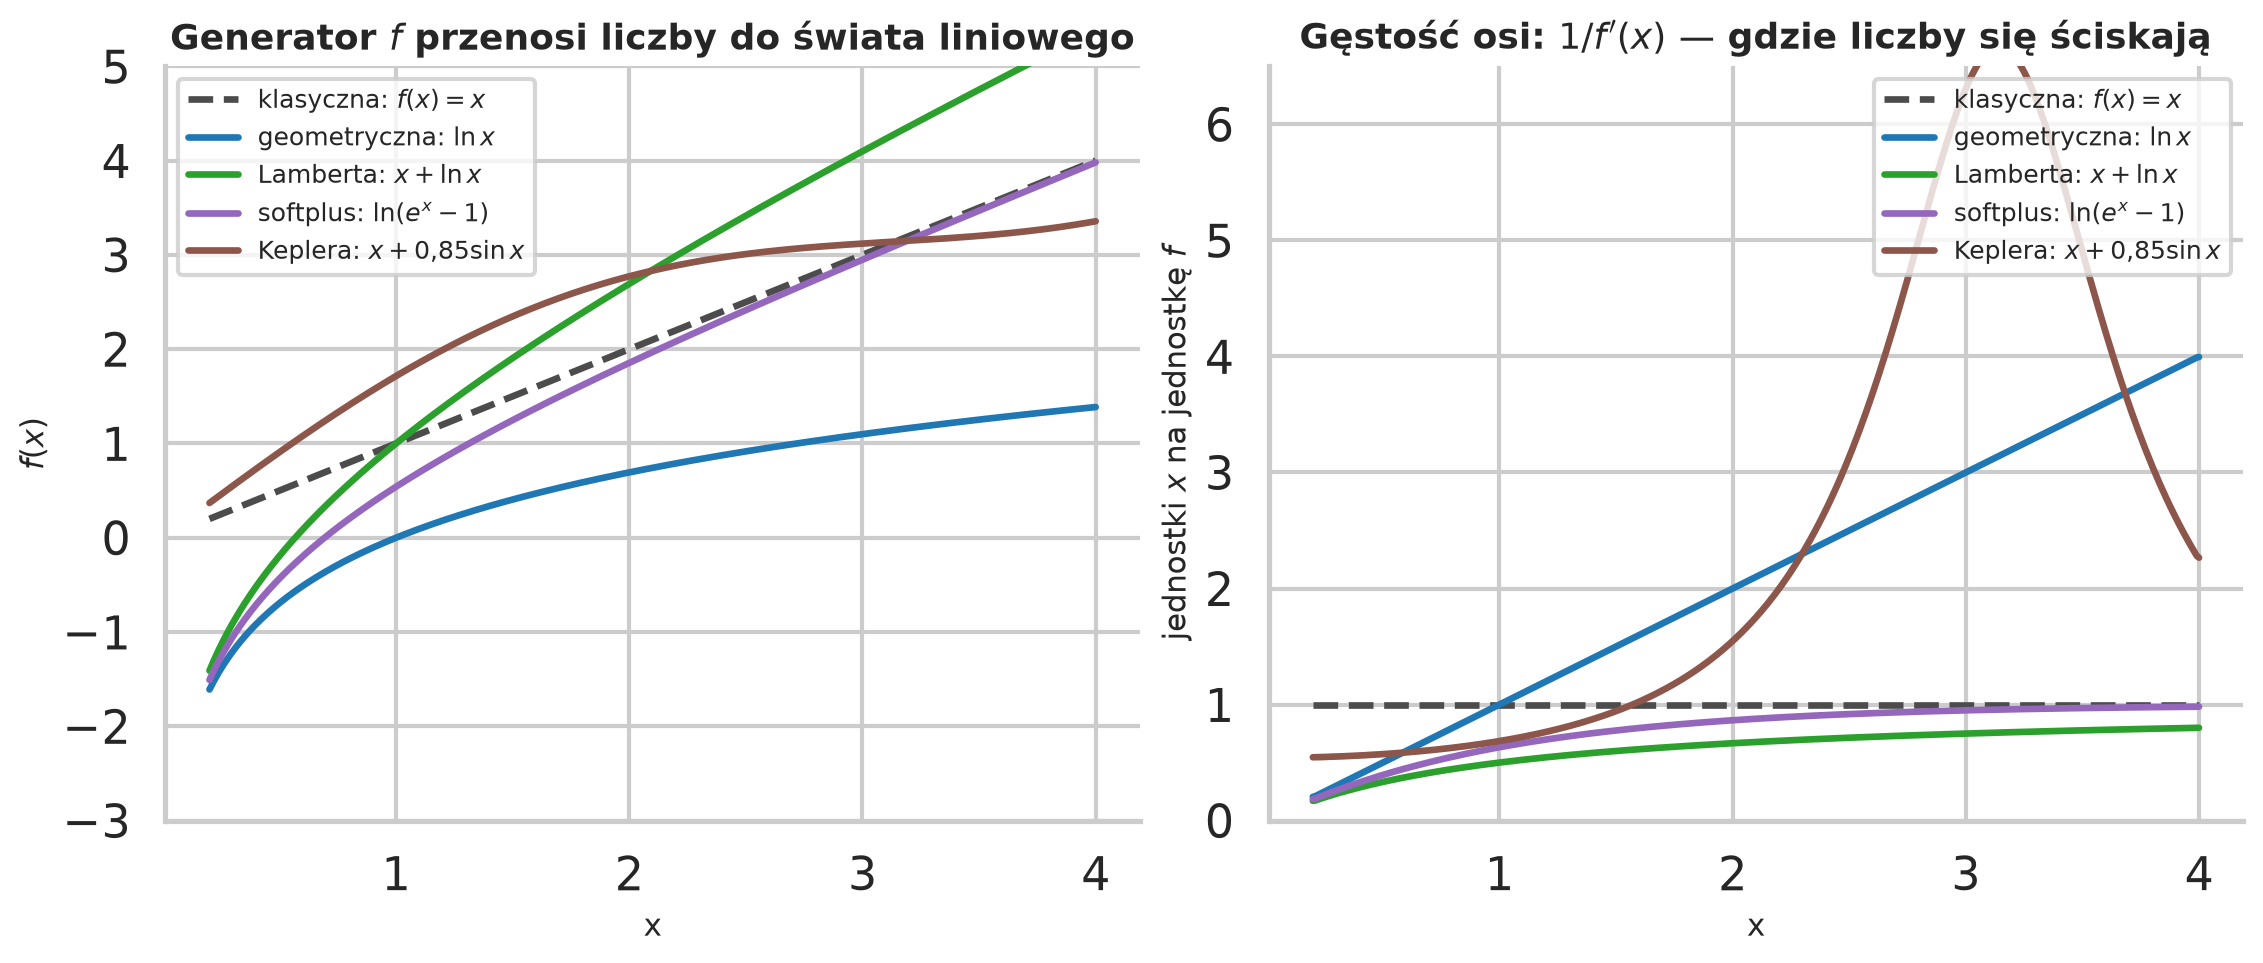
\includegraphics[width=\linewidth]{figures/fig01_generators.png}
\caption{Generator $f$ i gęstość osi $1/f'$. Wzrost $f'$ oznacza ściskanie
liczb, spadek -- rozciąganie.}\label{fig:gen}
\end{figure}

\begin{figure}[htbp]
\centering
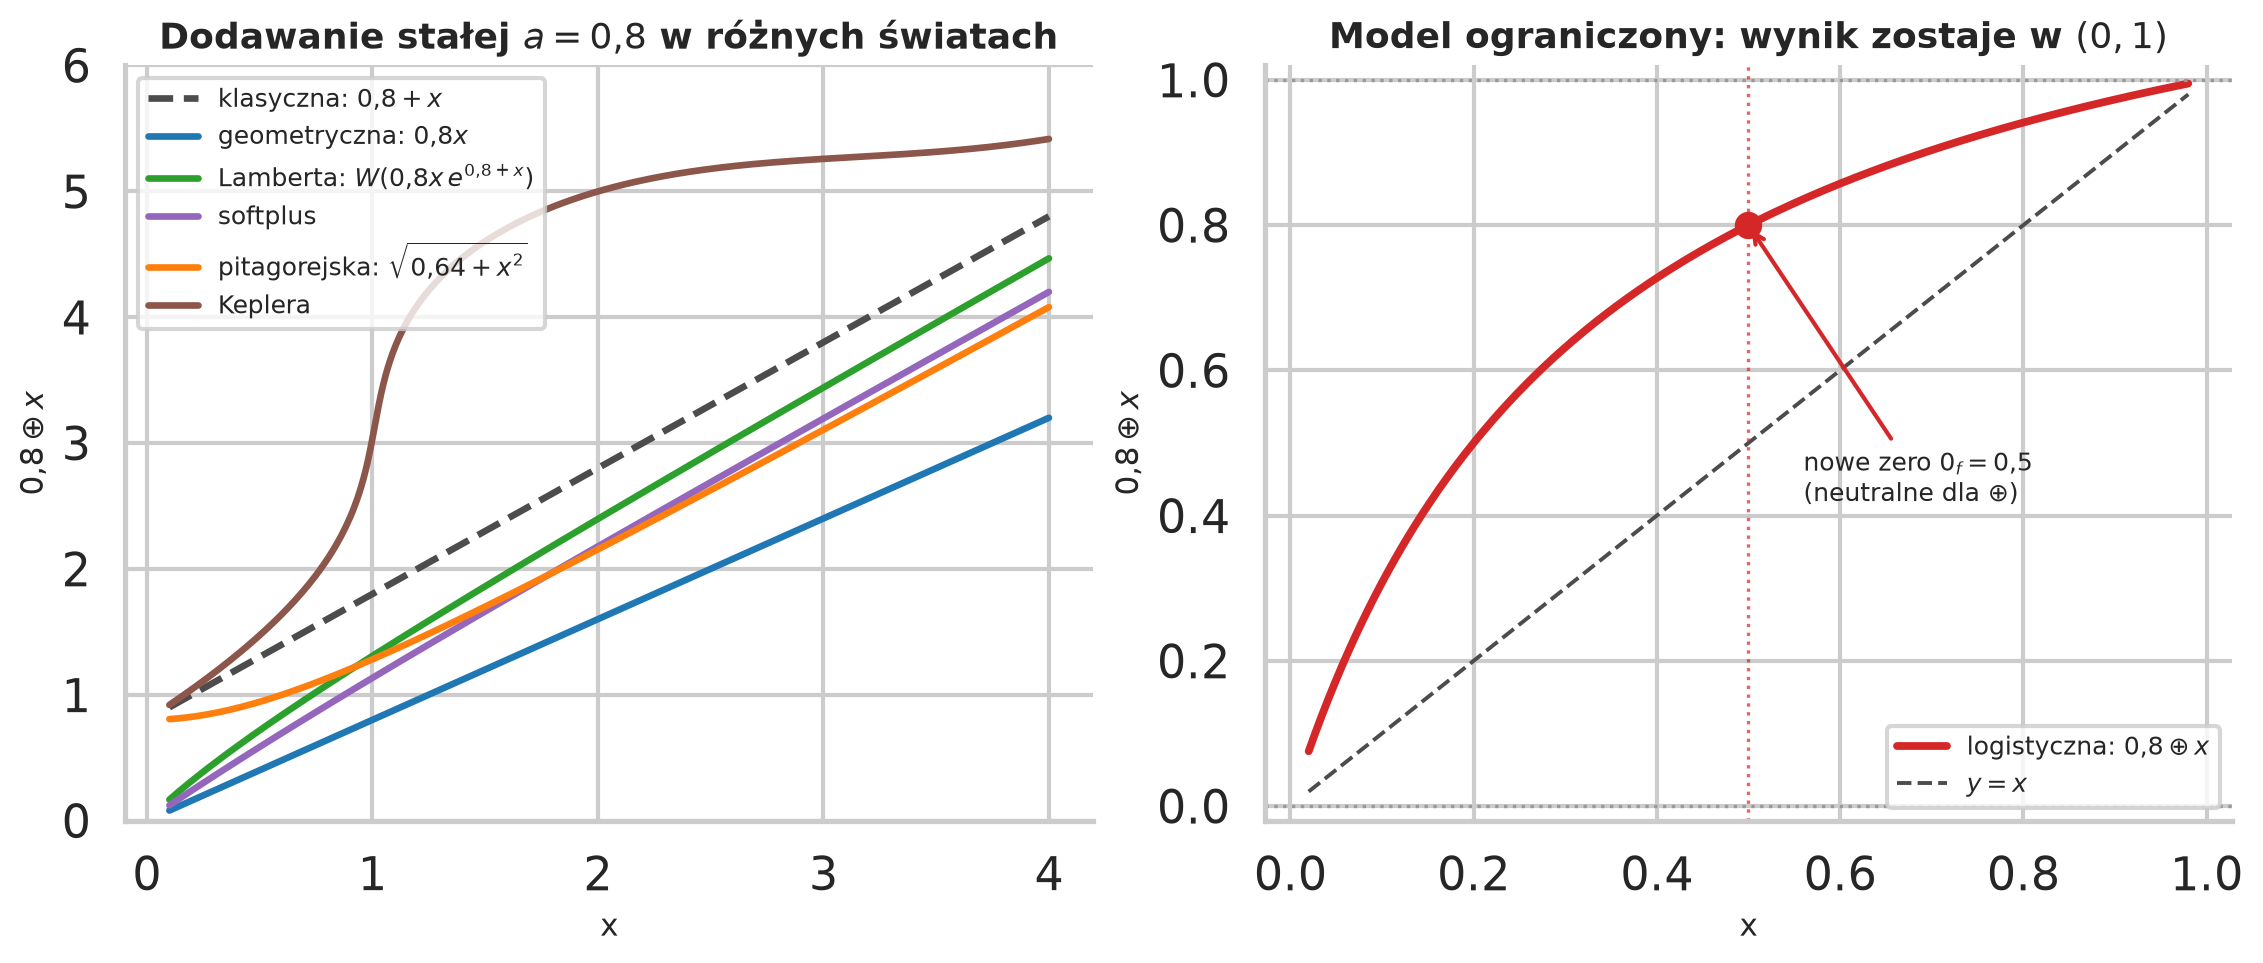
\includegraphics[width=\linewidth]{figures/fig02_addition.png}
\caption{To samo działanie $0{,}8\oplus x$ w siedmiu modelach; po prawej model
logistyczny z elementem neutralnym $0_f=0{,}5$.}\label{fig:add}
\end{figure}

\begin{figure}[htbp]
\centering
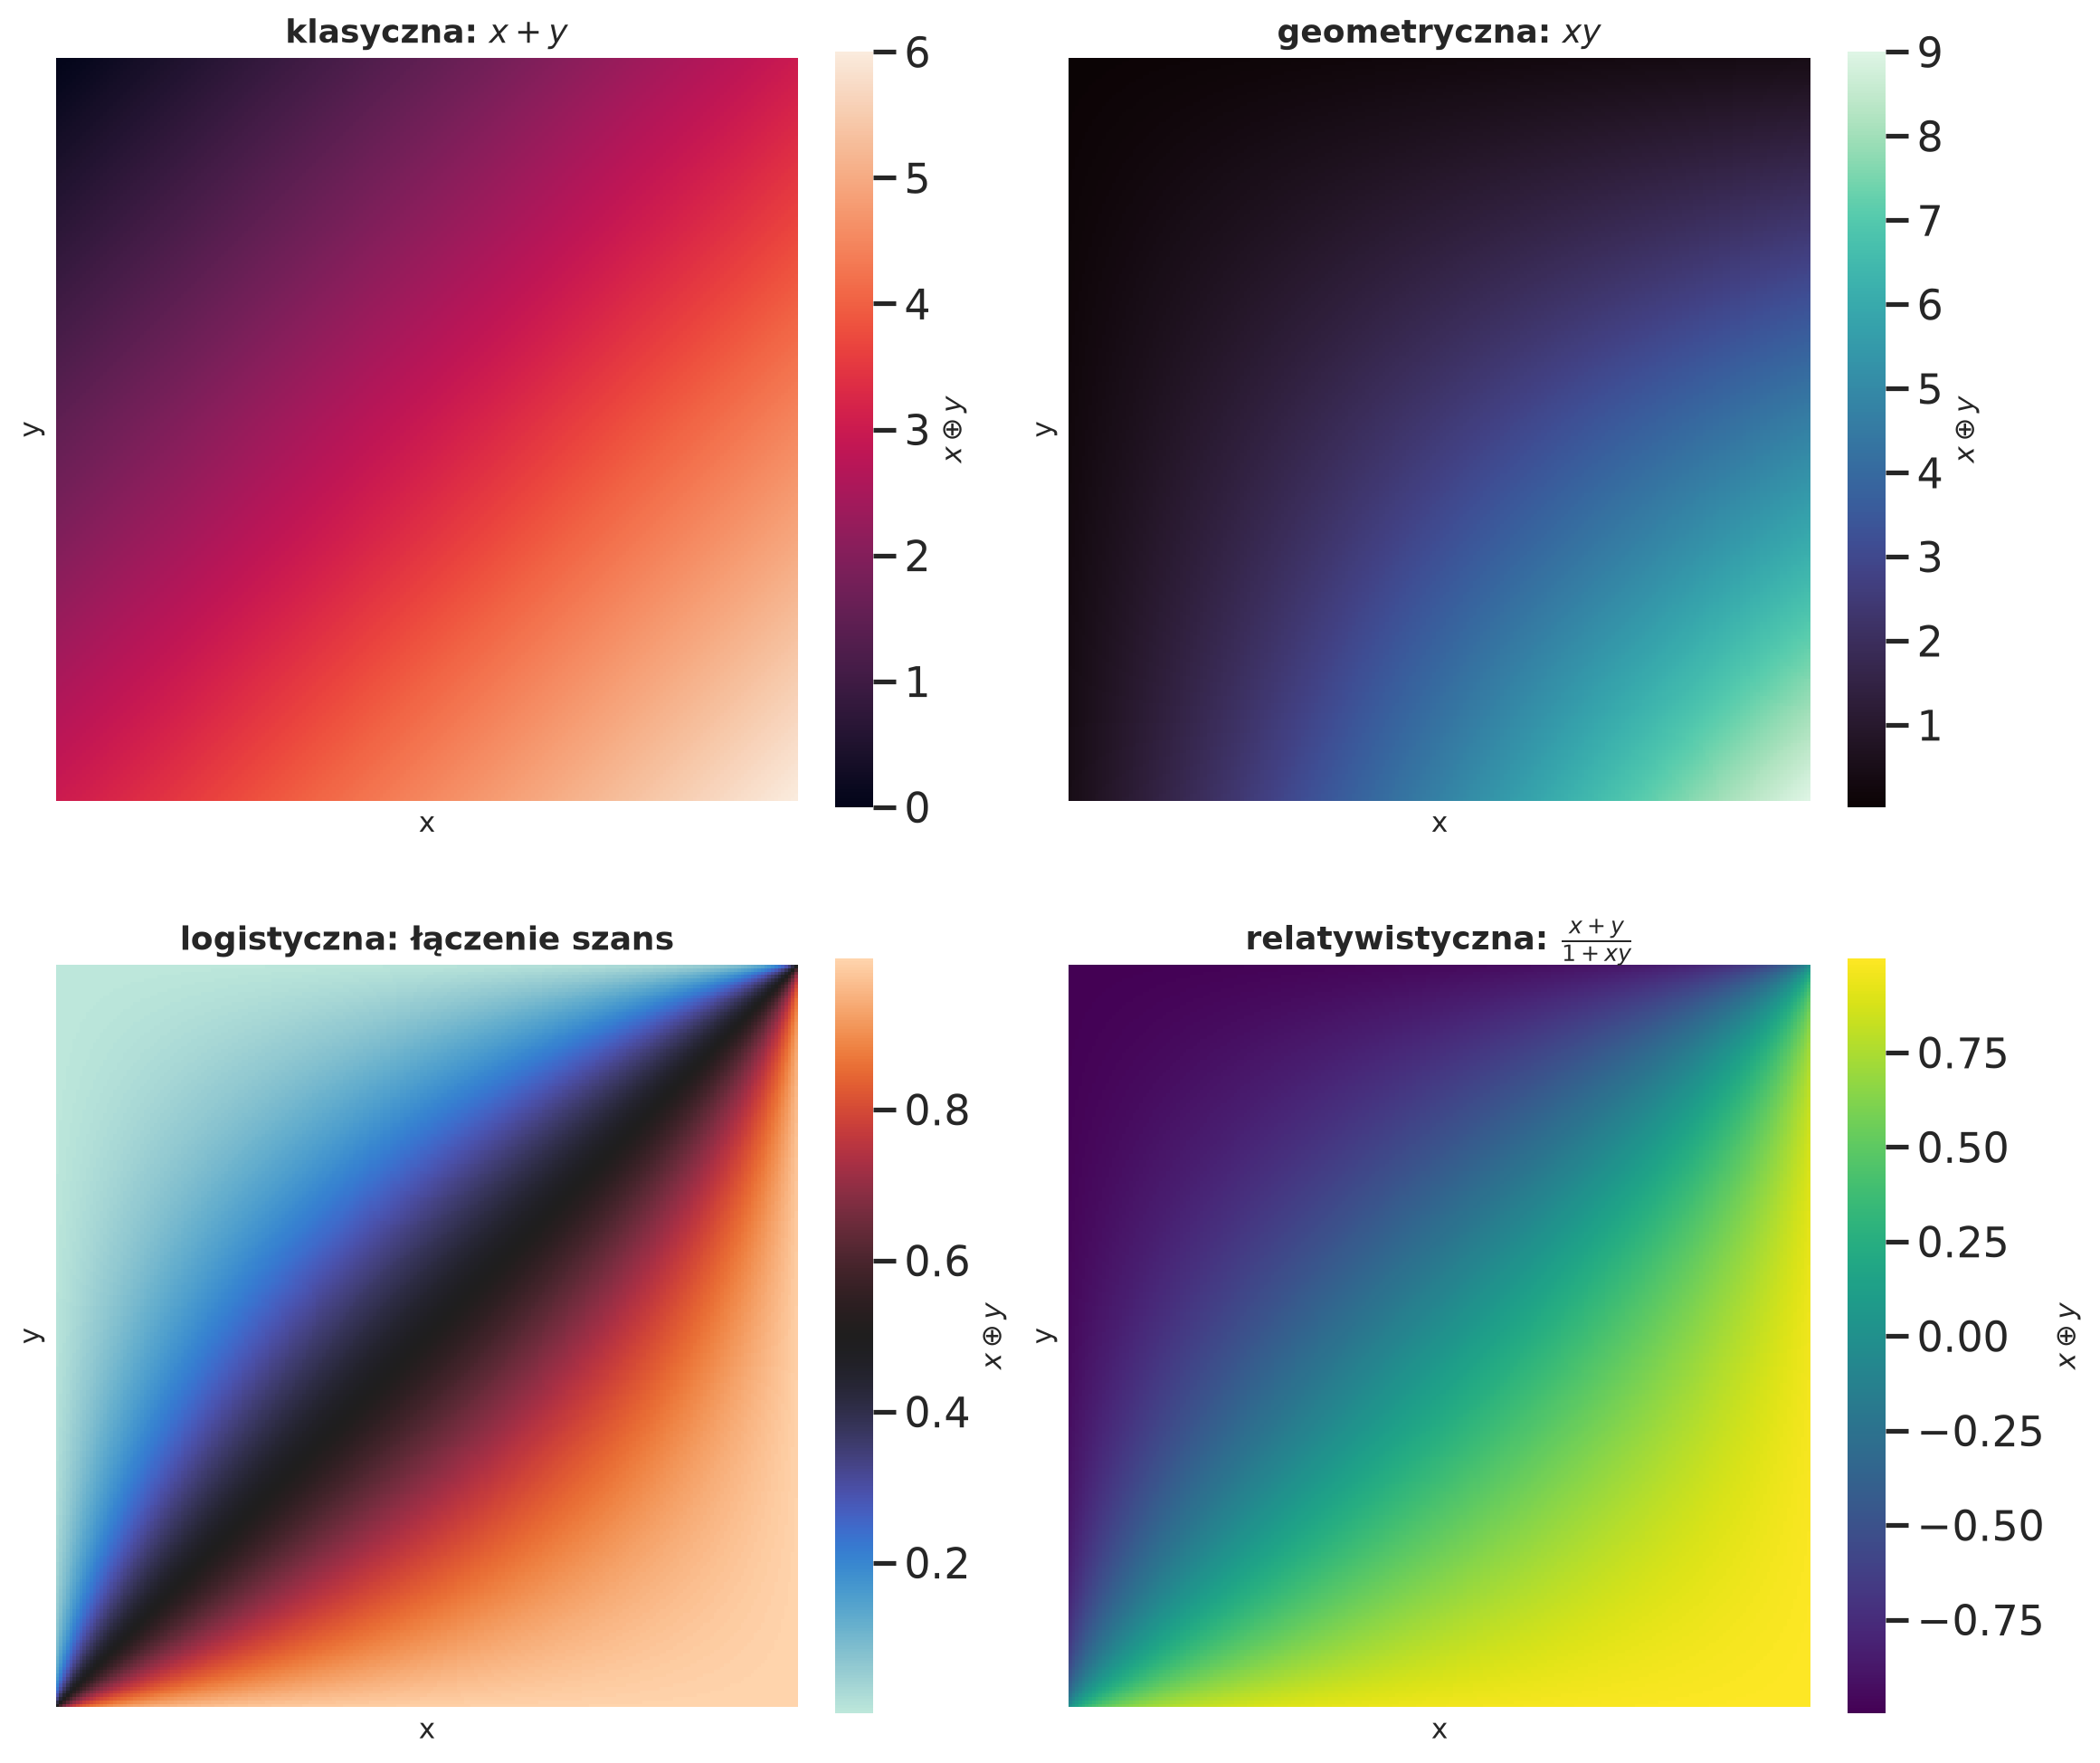
\includegraphics[width=\linewidth]{figures/fig03_heatmaps.png}
\caption{Mapy cieplne $z=x\oplus y$ dla czterech modeli.}\label{fig:heat}
\end{figure}

\begin{figure}[htbp]
\centering
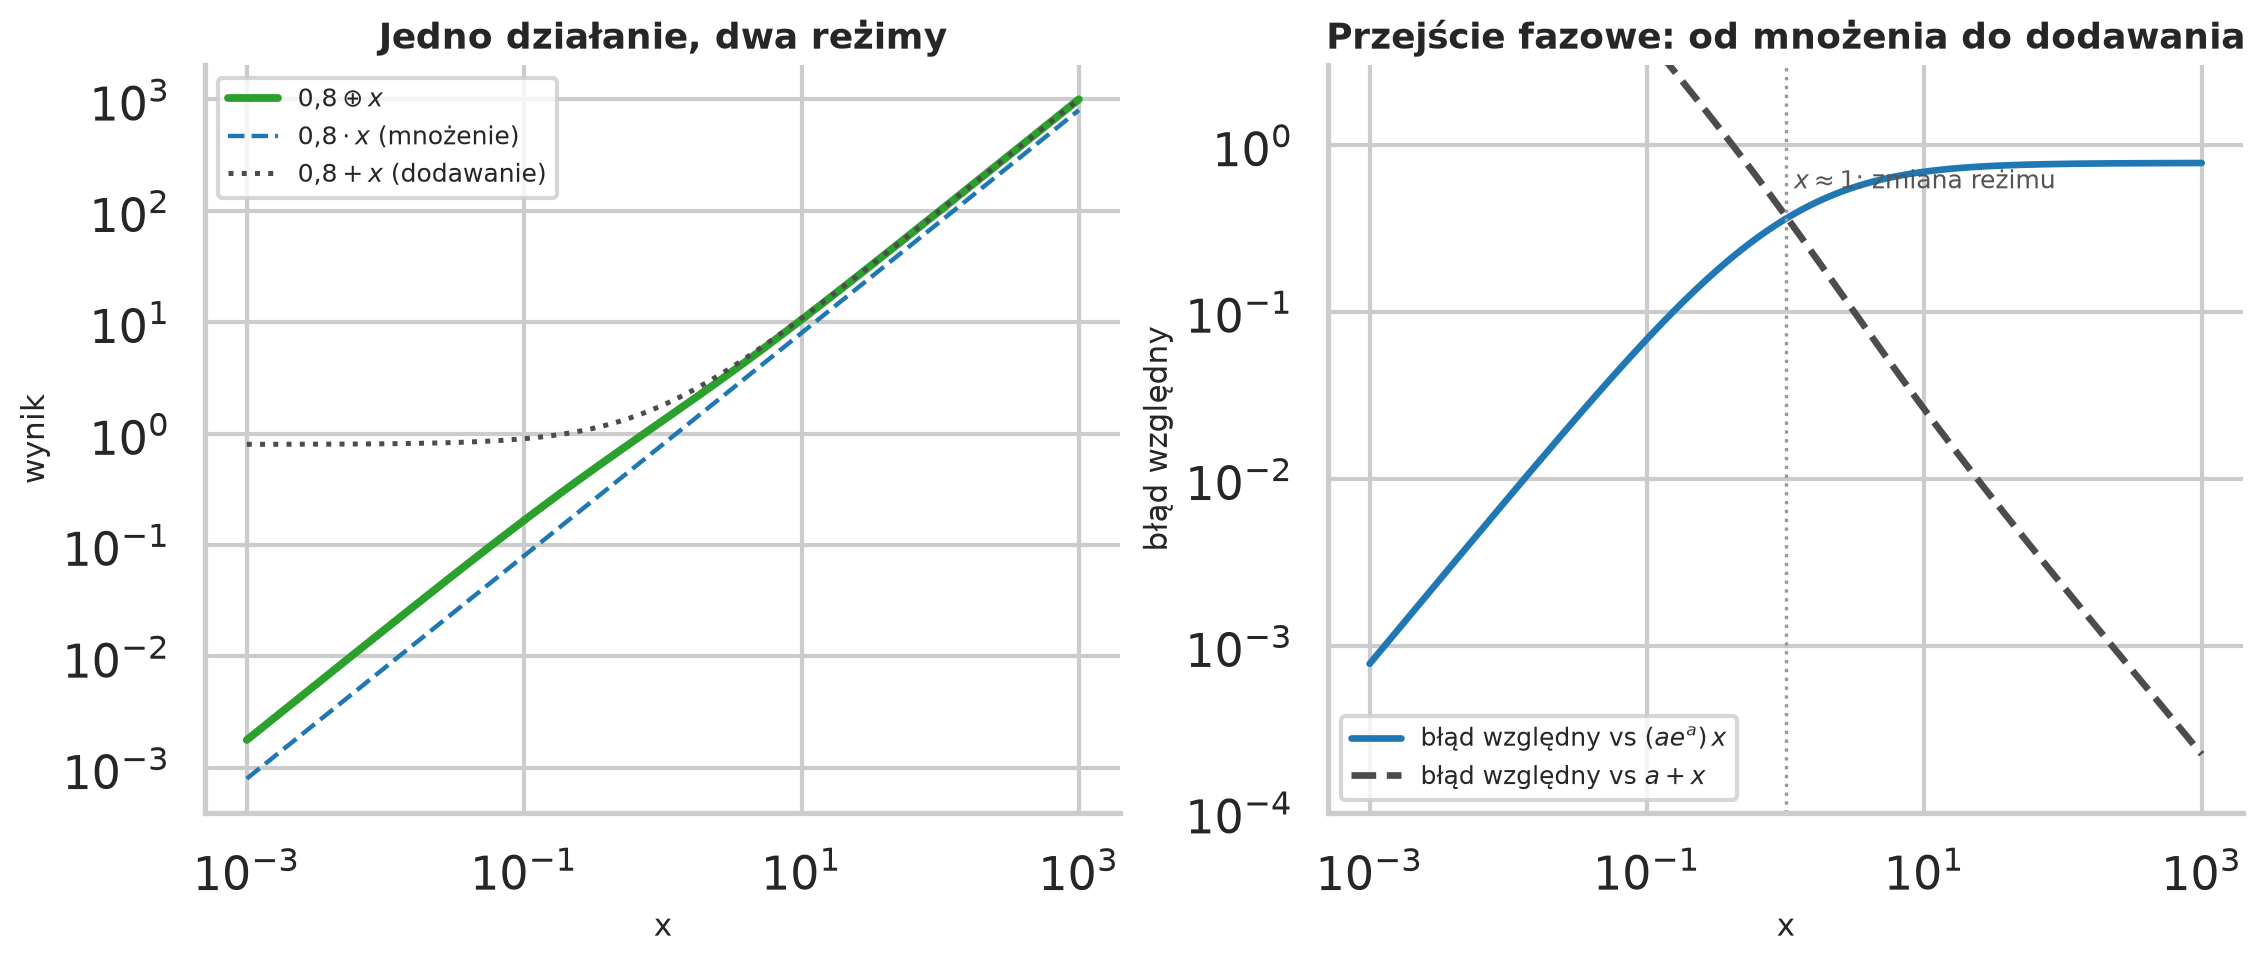
\includegraphics[width=\linewidth]{figures/fig04_phase_transition.png}
\caption{Model Lamberta: przejście od reżimu mnożenia do reżimu dodawania
wraz z błędami względnymi wobec obu asymptot.}\label{fig:phase}
\end{figure}

\begin{figure}[htbp]
\centering
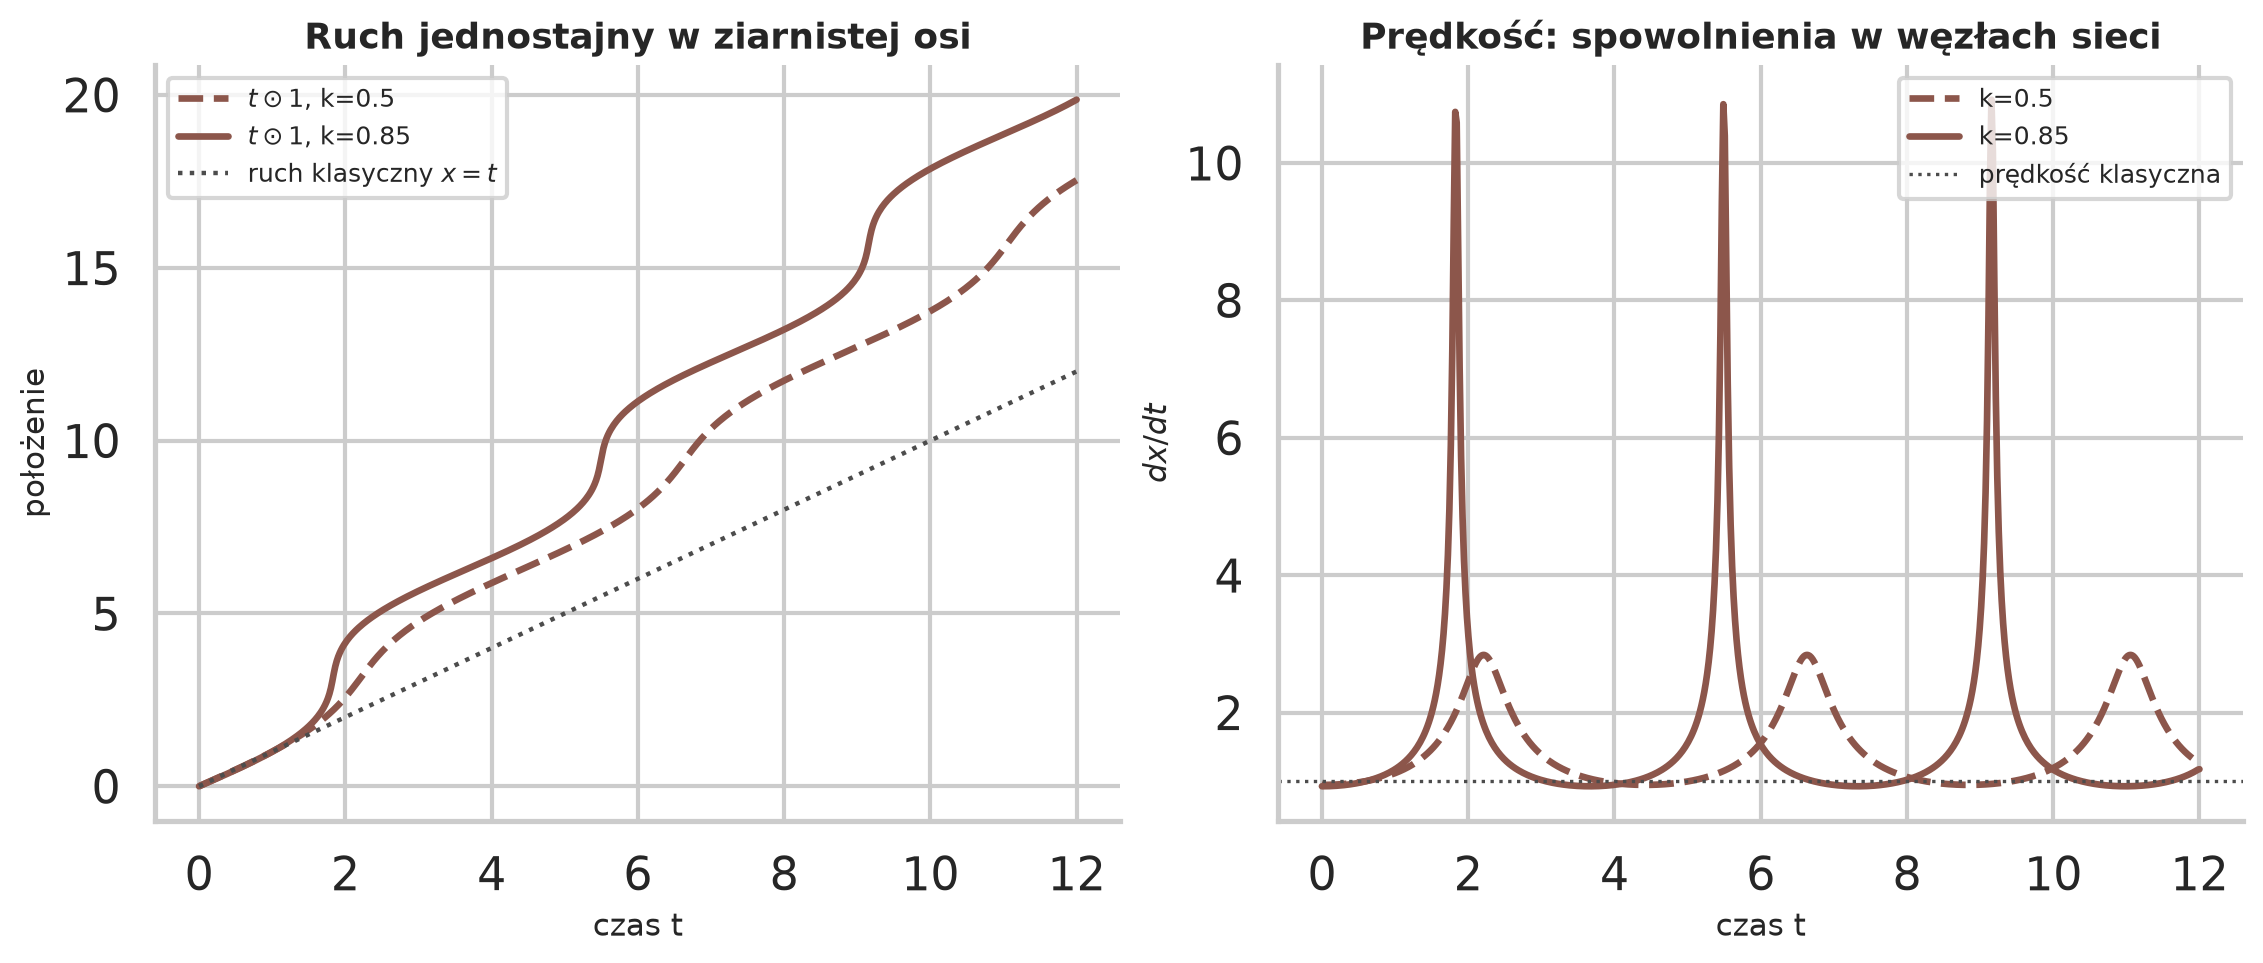
\includegraphics[width=\linewidth]{figures/fig05_kepler.png}
\caption{Ruch jednostajny w osi Keplera i jego prędkość; spowolnienia wypadają
w węzłach $x=(2n+1)\pi$.}\label{fig:kepler}
\end{figure}

\begin{figure}[htbp]
\centering
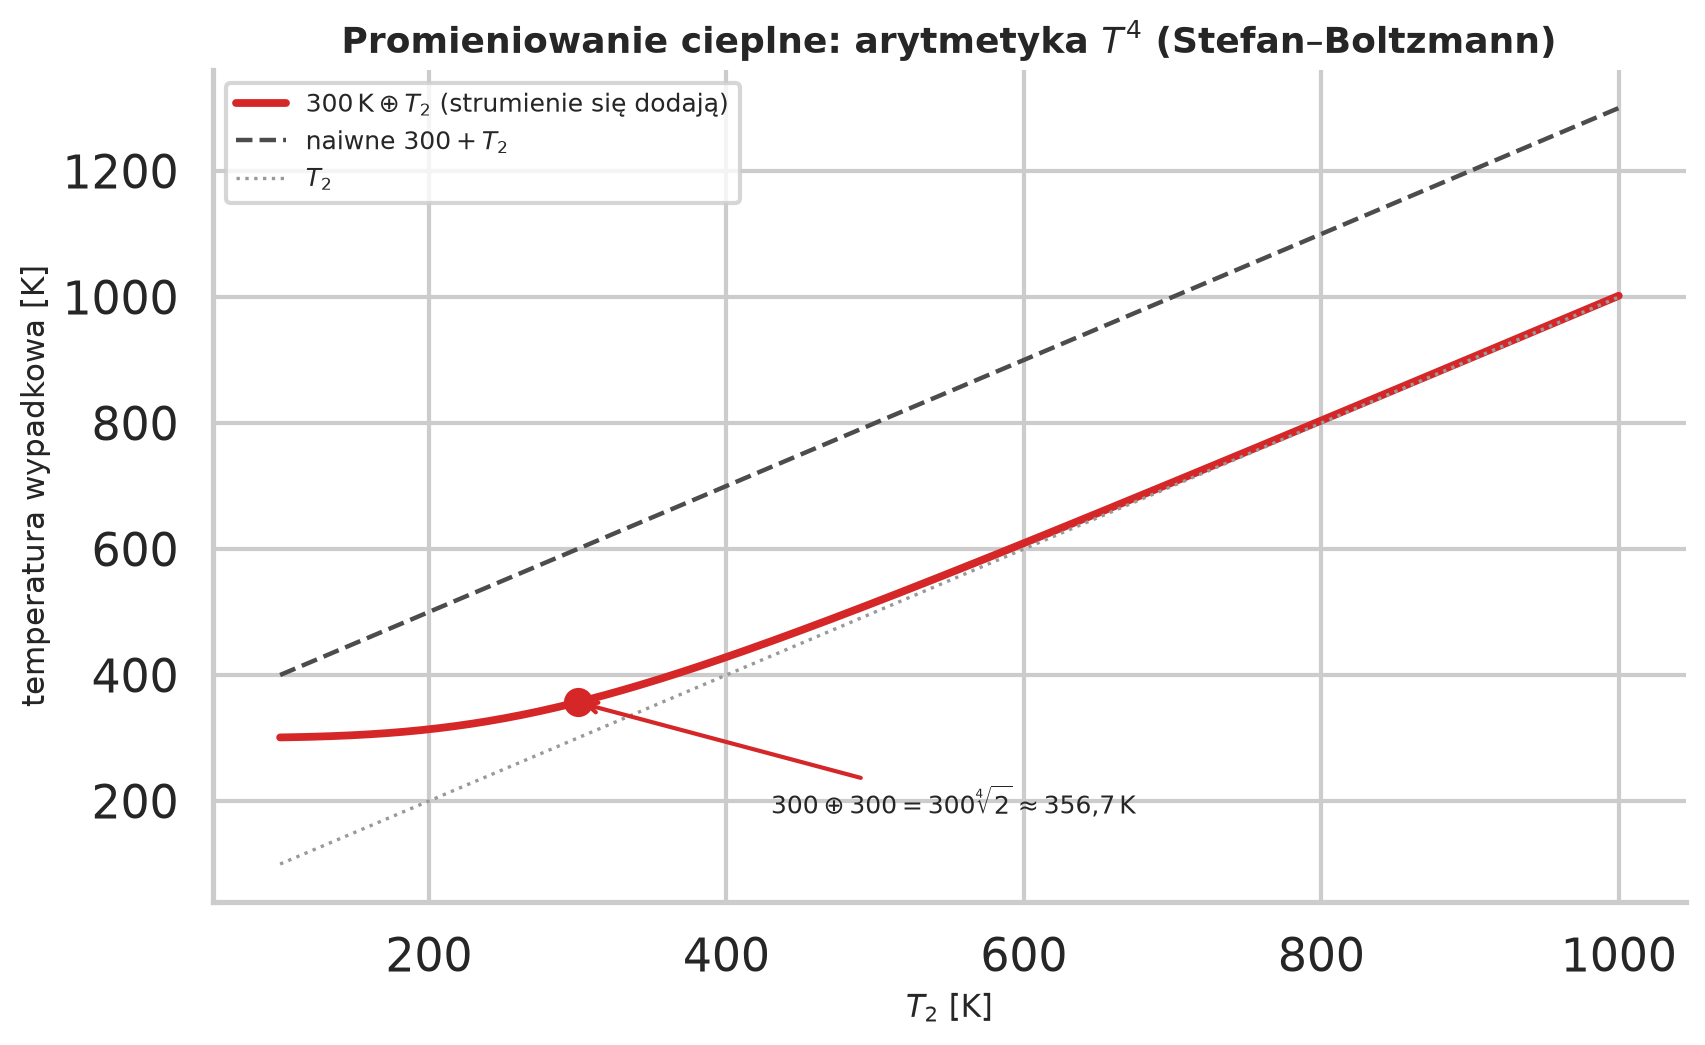
\includegraphics[width=0.86\linewidth]{figures/fig06_thermal_radiation.png}
\caption{Prawo Stefana--Boltzmanna jako arytmetyka $T^{4}$.}\label{fig:radiation}
\end{figure}

\begin{figure}[htbp]
\centering
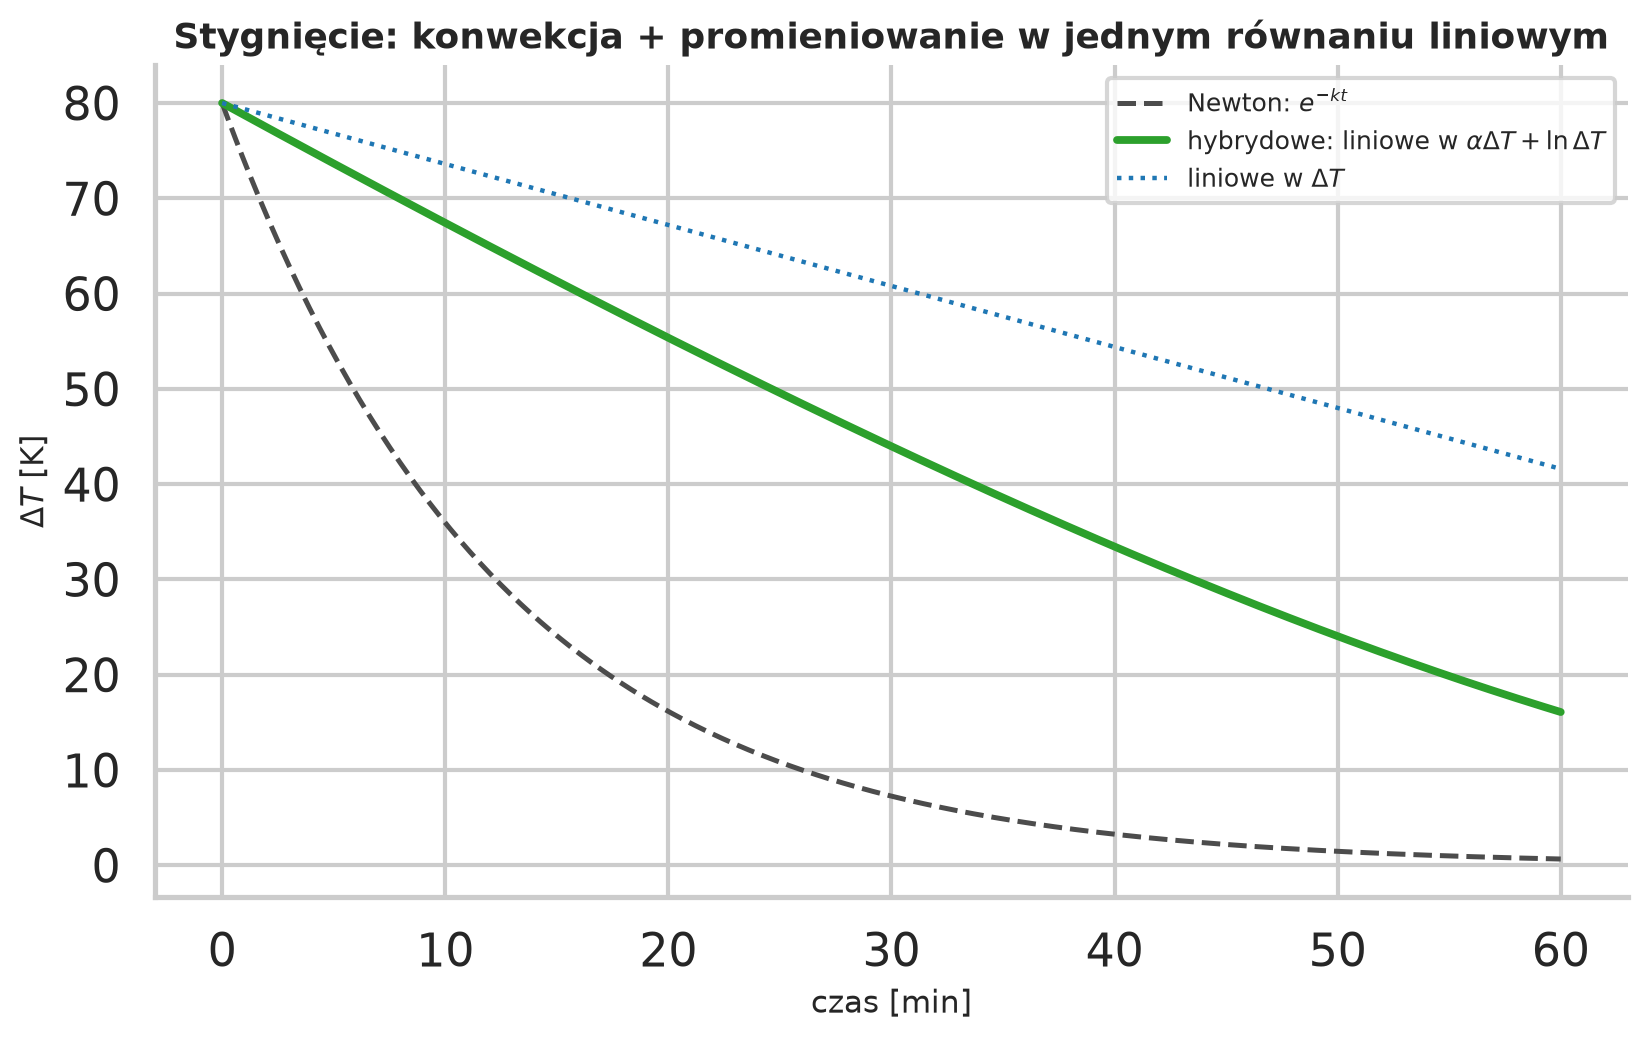
\includegraphics[width=0.86\linewidth]{figures/fig07_thermal_cooling.png}
\caption{Stygnięcie konwekcją i promieniowaniem: liniowe w zmiennej
$\alpha\Delta T+\ln\Delta T$, nieliniowe w $\Delta T$.}\label{fig:cooling}
\end{figure}

\begin{figure}[htbp]
\centering
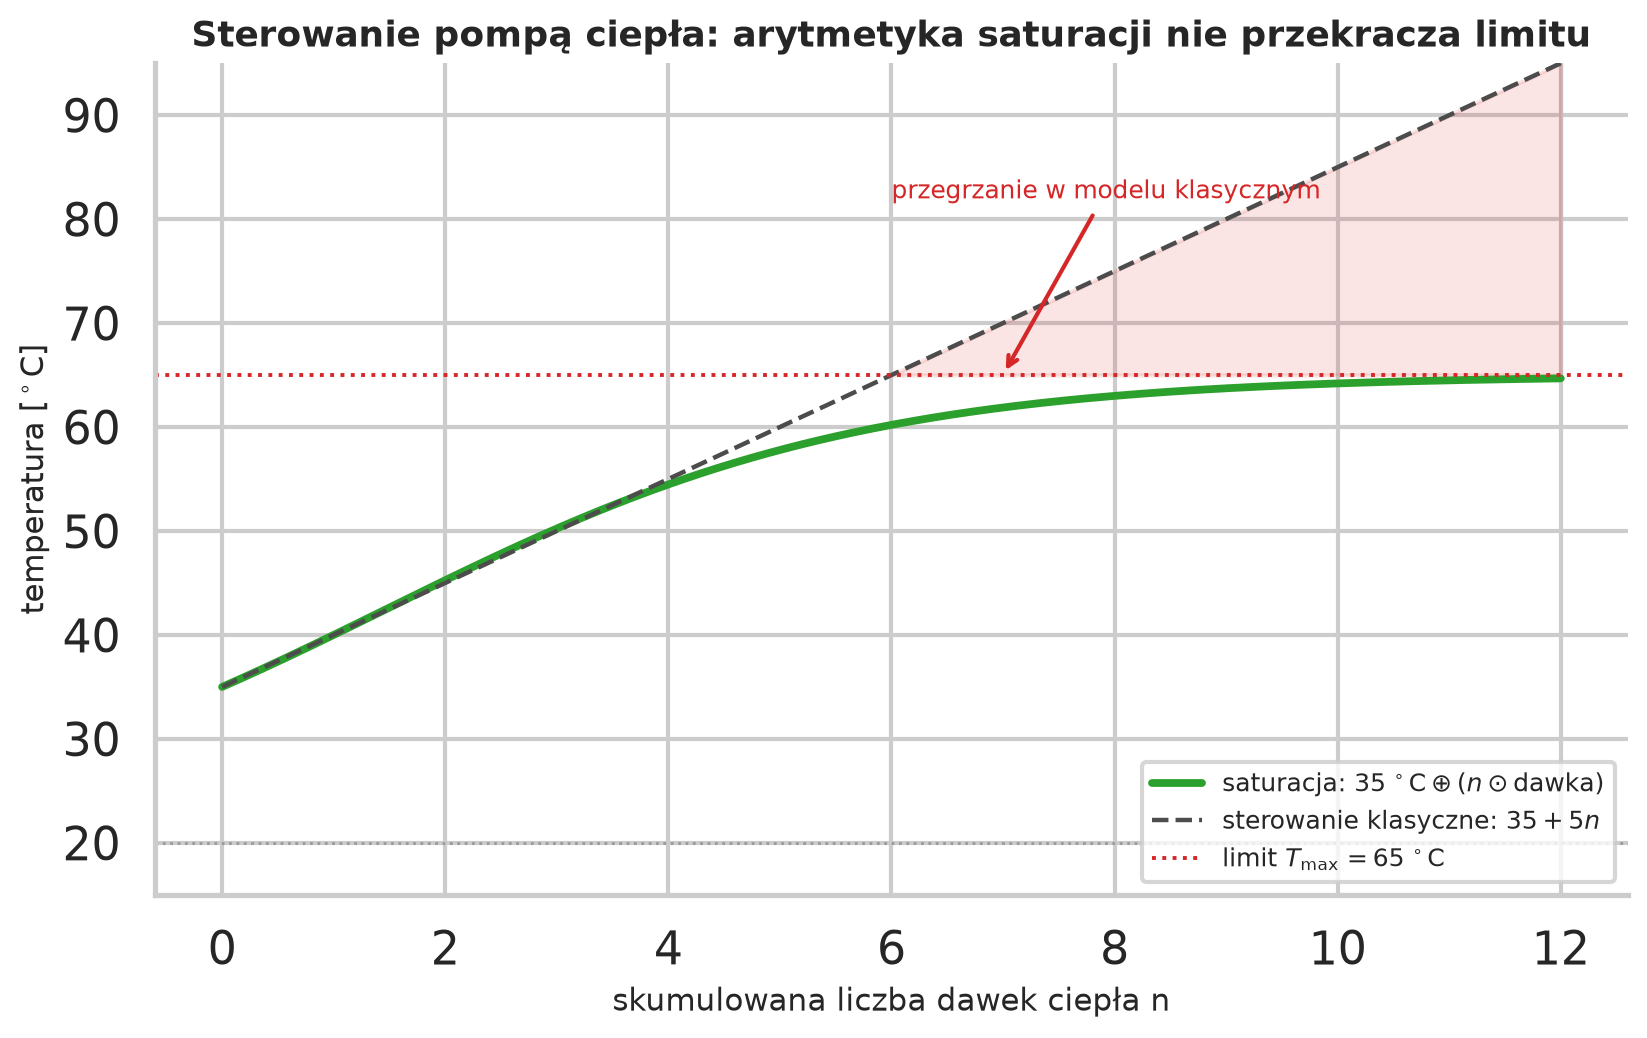
\includegraphics[width=0.86\linewidth]{figures/fig08_thermal_saturation.png}
\caption{Sterowanie z saturacją nie przekracza $T_{\max}$; sterowanie klasyczne
przegrzewa układ.}\label{fig:saturation}
\end{figure}

\begin{thebibliography}{9}
\bibitem{grossman1972} M. Grossman, R. Katz, \emph{Non-Newtonian Calculus},
Lee Press, Pigeon Cove, 1972.
\bibitem{einstein1905} A. Einstein, Zur Elektrodynamik bewegter Körper,
\emph{Annalen der Physik} 17 (1905), 891--921.
\bibitem{kolmogorov1930} A. Kolmogorov, Sur la notion de la moyenne,
\emph{Atti Accad. Naz. Lincei} 12 (1930), 388--391.
\bibitem{nagumo1930} M. Nagumo, Über eine Klasse von Mittelbildungen mit
Anwendungen auf die Differentialgeometrie, \emph{Japanese J. Math.} 7 (1930).
\bibitem{corless1996} R. Corless, G. Gonnet, D. Hare, D. Jeffrey, D. Knuth,
On the Lambert $W$ function, \emph{Adv. Comput. Math.} 5 (1996), 329--359.
\bibitem{kepler1609} J. Kepler, \emph{Astronomia nova}, Praga, 1609.
\end{thebibliography}

\end{document}
